\section{Tersinir Sistemler}

\begin{justify}
Birçok mekanik sistem zaman tersinim simetrisine sahiptir. Bu, zaman ileri ya da geri aksa da sistemin dinamiğinin aynı görünmesi anlamına gelir. Örneğin sönümsüz bir sarkacın ileri geri salındığı bir filmi geriye doğru izlerseniz fiziksel olarak saçma bir durum görmezsiniz.

Aslında
\begin{equation}
m\ddot{x}=F(x)
\end{equation}
biçimindeki her mekanik sistem zaman tersinimi altında simetriktir. $t\mapsto -t$ değişken dönüşümü yapılırsa ikinci türev $\ddot{x}$ değişmez ve denklem aynı kalır. Elbette hız $\dot{x}$ işaret değiştirir. Bunun faz düzleminde ne anlama geldiğini görmek için eşdeğer sistemi yazalım:
\begin{align}
\dot{x} &= y,\\
\dot{y} &= \frac{1}{m}F(x),
\end{align}
burada $y$ hızdır. $t\mapsto -t$ ve $y\mapsto -y$ dönüşümleri yapılırsa iki denklem de aynı kalır. Dolayısıyla $(x(t),y(t))$ bir çözümse, $(x(-t),-y(-t))$ de bir çözümdür. Bu nedenle her yörüngenin bir ikizi vardır: bu iki yörünge yalnızca zamanın ters çevrilmesi ve $x$ eksenine göre yansıma bakımından farklıdır (Şekil~\ref{fig:6-6-1}).

\begin{figure}[H]
\centering
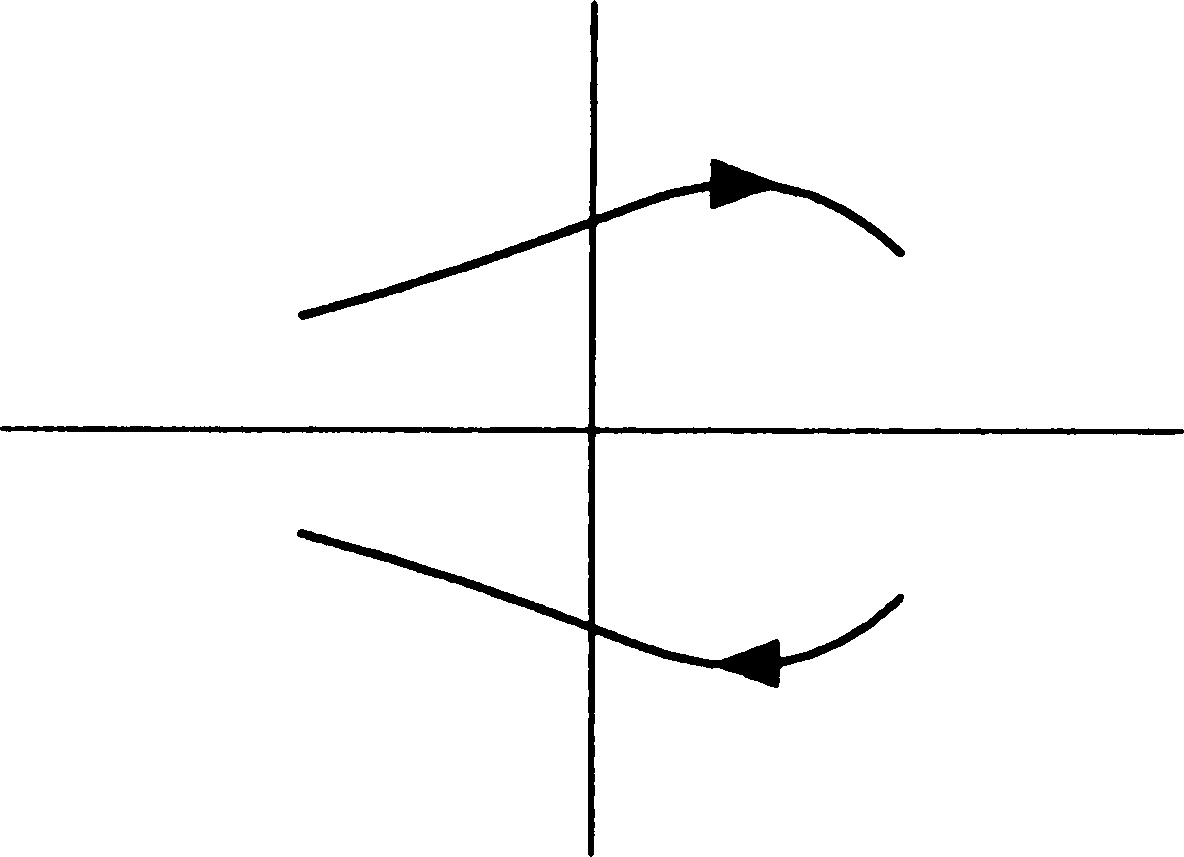
\includegraphics[width=0.82\textwidth]{images/Figures/figur-020.png}
\caption{Tersinir sistemde yörüngenin $x$ eksenine göre yansıyan ikizi.}
\label{fig:6-6-1}
\end{figure}

Genel olarak, $t\mapsto -t$ ve $y\mapsto -y$ altında değişmeyen her ikinci mertebeden sistemi tersinir sistem olarak tanımlayalım. Örneğin
\begin{align}
\dot{x} &= f(x,y),\\
\dot{y} &= g(x,y)
\end{align}
biçimindeki bir sistemde $f$ fonksiyonu $y$ değişkenine göre tek, $g$ fonksiyonu ise $y$ değişkenine göre çift ise sistem tersinirdir; yani
\begin{equation}
f(x,-y)=-f(x,y), \qquad g(x,-y)=g(x,y).
\end{equation}

Tersinir sistemler korunumlu sistemlerden farklıdır; fakat onların birçok özelliğine sahiptir. Örneğin aşağıdaki teorem, merkezlerin tersinir sistemlerde de dayanıklı olduğunu gösterir.

\textbf{Teorem 6.6.1.} Orijin, sürekli türevlenebilir
\begin{align}
\dot{x} &= f(x,y),\\
\dot{y} &= g(x,y)
\end{align}
sistemi için doğrusal bir merkez olsun ve sistem tersinir olsun. O zaman orijine yeterince yakın tüm yörüngeler kapalı eğrilerdir.

\textbf{İspat fikri.} Orijine yakın pozitif $x$ ekseni üzerinde başlayan bir yörünge düşünelim (Şekil~\ref{fig:6-6-2}). Orijine yeterince yakın bölgede doğrusal merkezin baskın etkisi nedeniyle akış orijin çevresinde döner ve yörünge sonunda negatif $x$ eksenini keser. Şimdi tersinirlik kullanılır. Yörünge $x$ eksenine göre yansıtılır ve zamanın işareti değiştirilirse, aynı uç noktalara sahip fakat oku ters yönde olan ikiz bir yörünge elde edilir (Şekil~\ref{fig:6-6-3}). Bu iki yörünge birlikte kapalı bir yörünge oluşturur.

\begin{figure}[H]
\centering
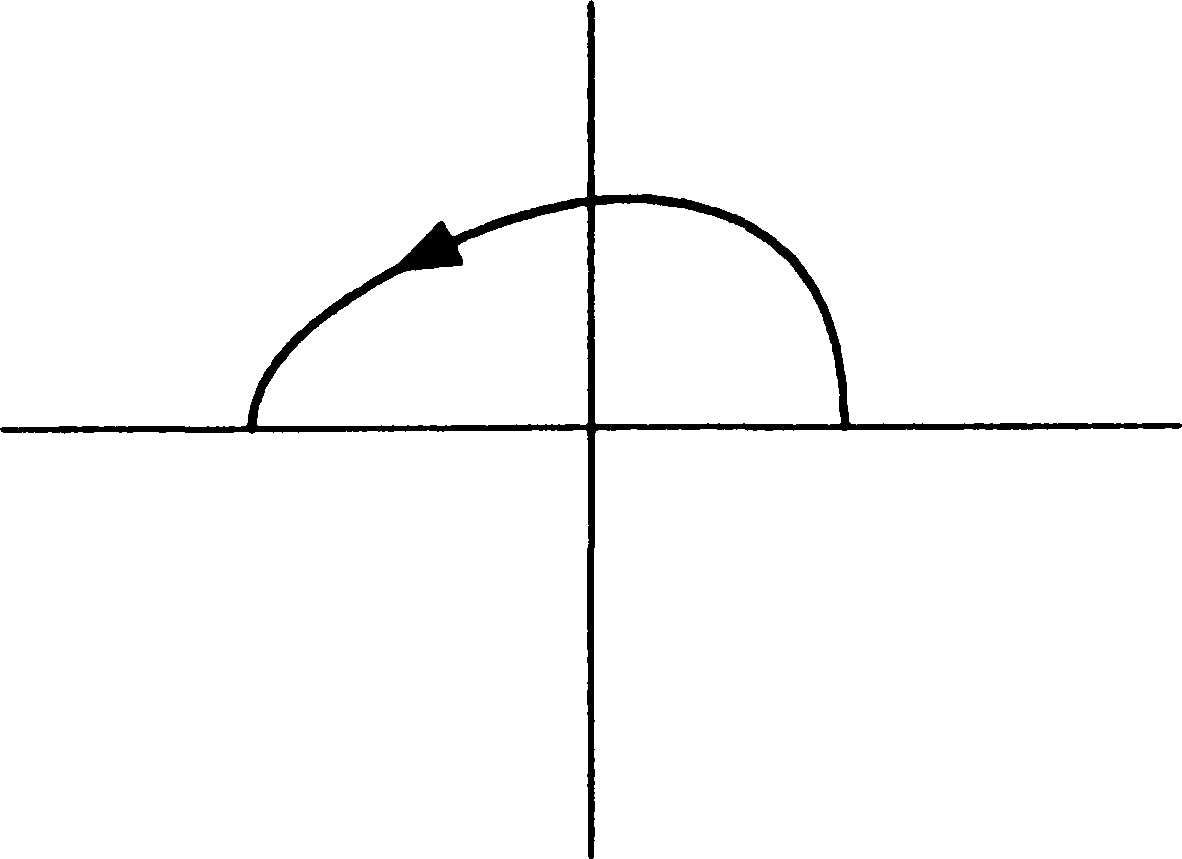
\includegraphics[width=0.82\textwidth]{images/Figures/figur-021.png}
\caption{Pozitif $x$ ekseninden başlayan yörüngenin negatif $x$ eksenini kesmesi.}
\label{fig:6-6-2}
\end{figure}
\begin{figure}[H]
\centering
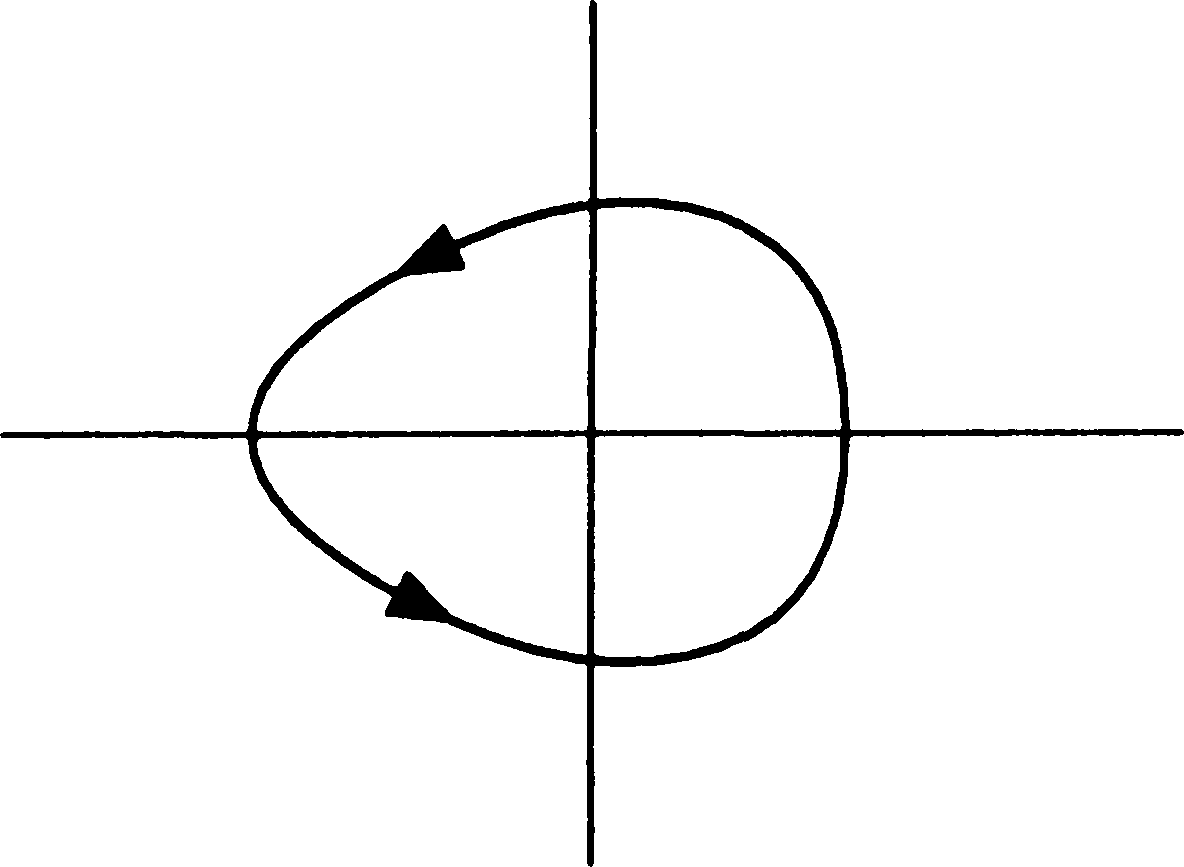
\includegraphics[width=0.82\textwidth]{images/Figures/figur-022.png}
\caption{Tersinirlik ile elde edilen ikiz yörünge ve kapalı eğri.}
\label{fig:6-6-3}
\end{figure}
\end{justify}

\subsection*{Örnek 6.6.1}
\addcontentsline{toc}{subsection}{Örnek 6.6.1}

\begin{justify}
Aşağıdaki sistemin orijinde doğrusal olmayan bir merkeze sahip olduğunu gösterin ve faz portresini çizin:
\begin{align}
\dot{x} &= y-y^3,\\
\dot{y} &= -x-y^2.
\end{align}

\textbf{Çözüm.} Teoremin varsayımlarının sağlandığını göstereceğiz. Orijindeki Jacobian matrisi
\begin{equation}
A=\begin{pmatrix}0&1\\-1&0\end{pmatrix}
\end{equation}
olur. Bu matris için $\tau=0$ ve $\Delta>0$ olduğundan orijin doğrusal bir merkezdir. Ayrıca sistem $t\mapsto -t$, $y\mapsto -y$ dönüşümü altında değişmediği için tersinirdir. Teorem 6.6.1'e göre orijin doğrusal olmayan bir merkezdir.

Sistemin diğer sabit noktaları $(-1,1)$ ve $(-1,-1)$ noktalarıdır. Lineerleştirme ile kolayca kontrol edilebileceği gibi bunlar eyer noktalarıdır. Bilgisayar üretimli faz portresi Şekil~\ref{fig:6-6-4}'te gösterilecektir. Tersinirlik simetrisi açıktır: $x$ ekseninin üstündeki yörüngelerin, okları ters yönde olacak şekilde altında ikizleri bulunur.

\begin{figure}[H]
\centering
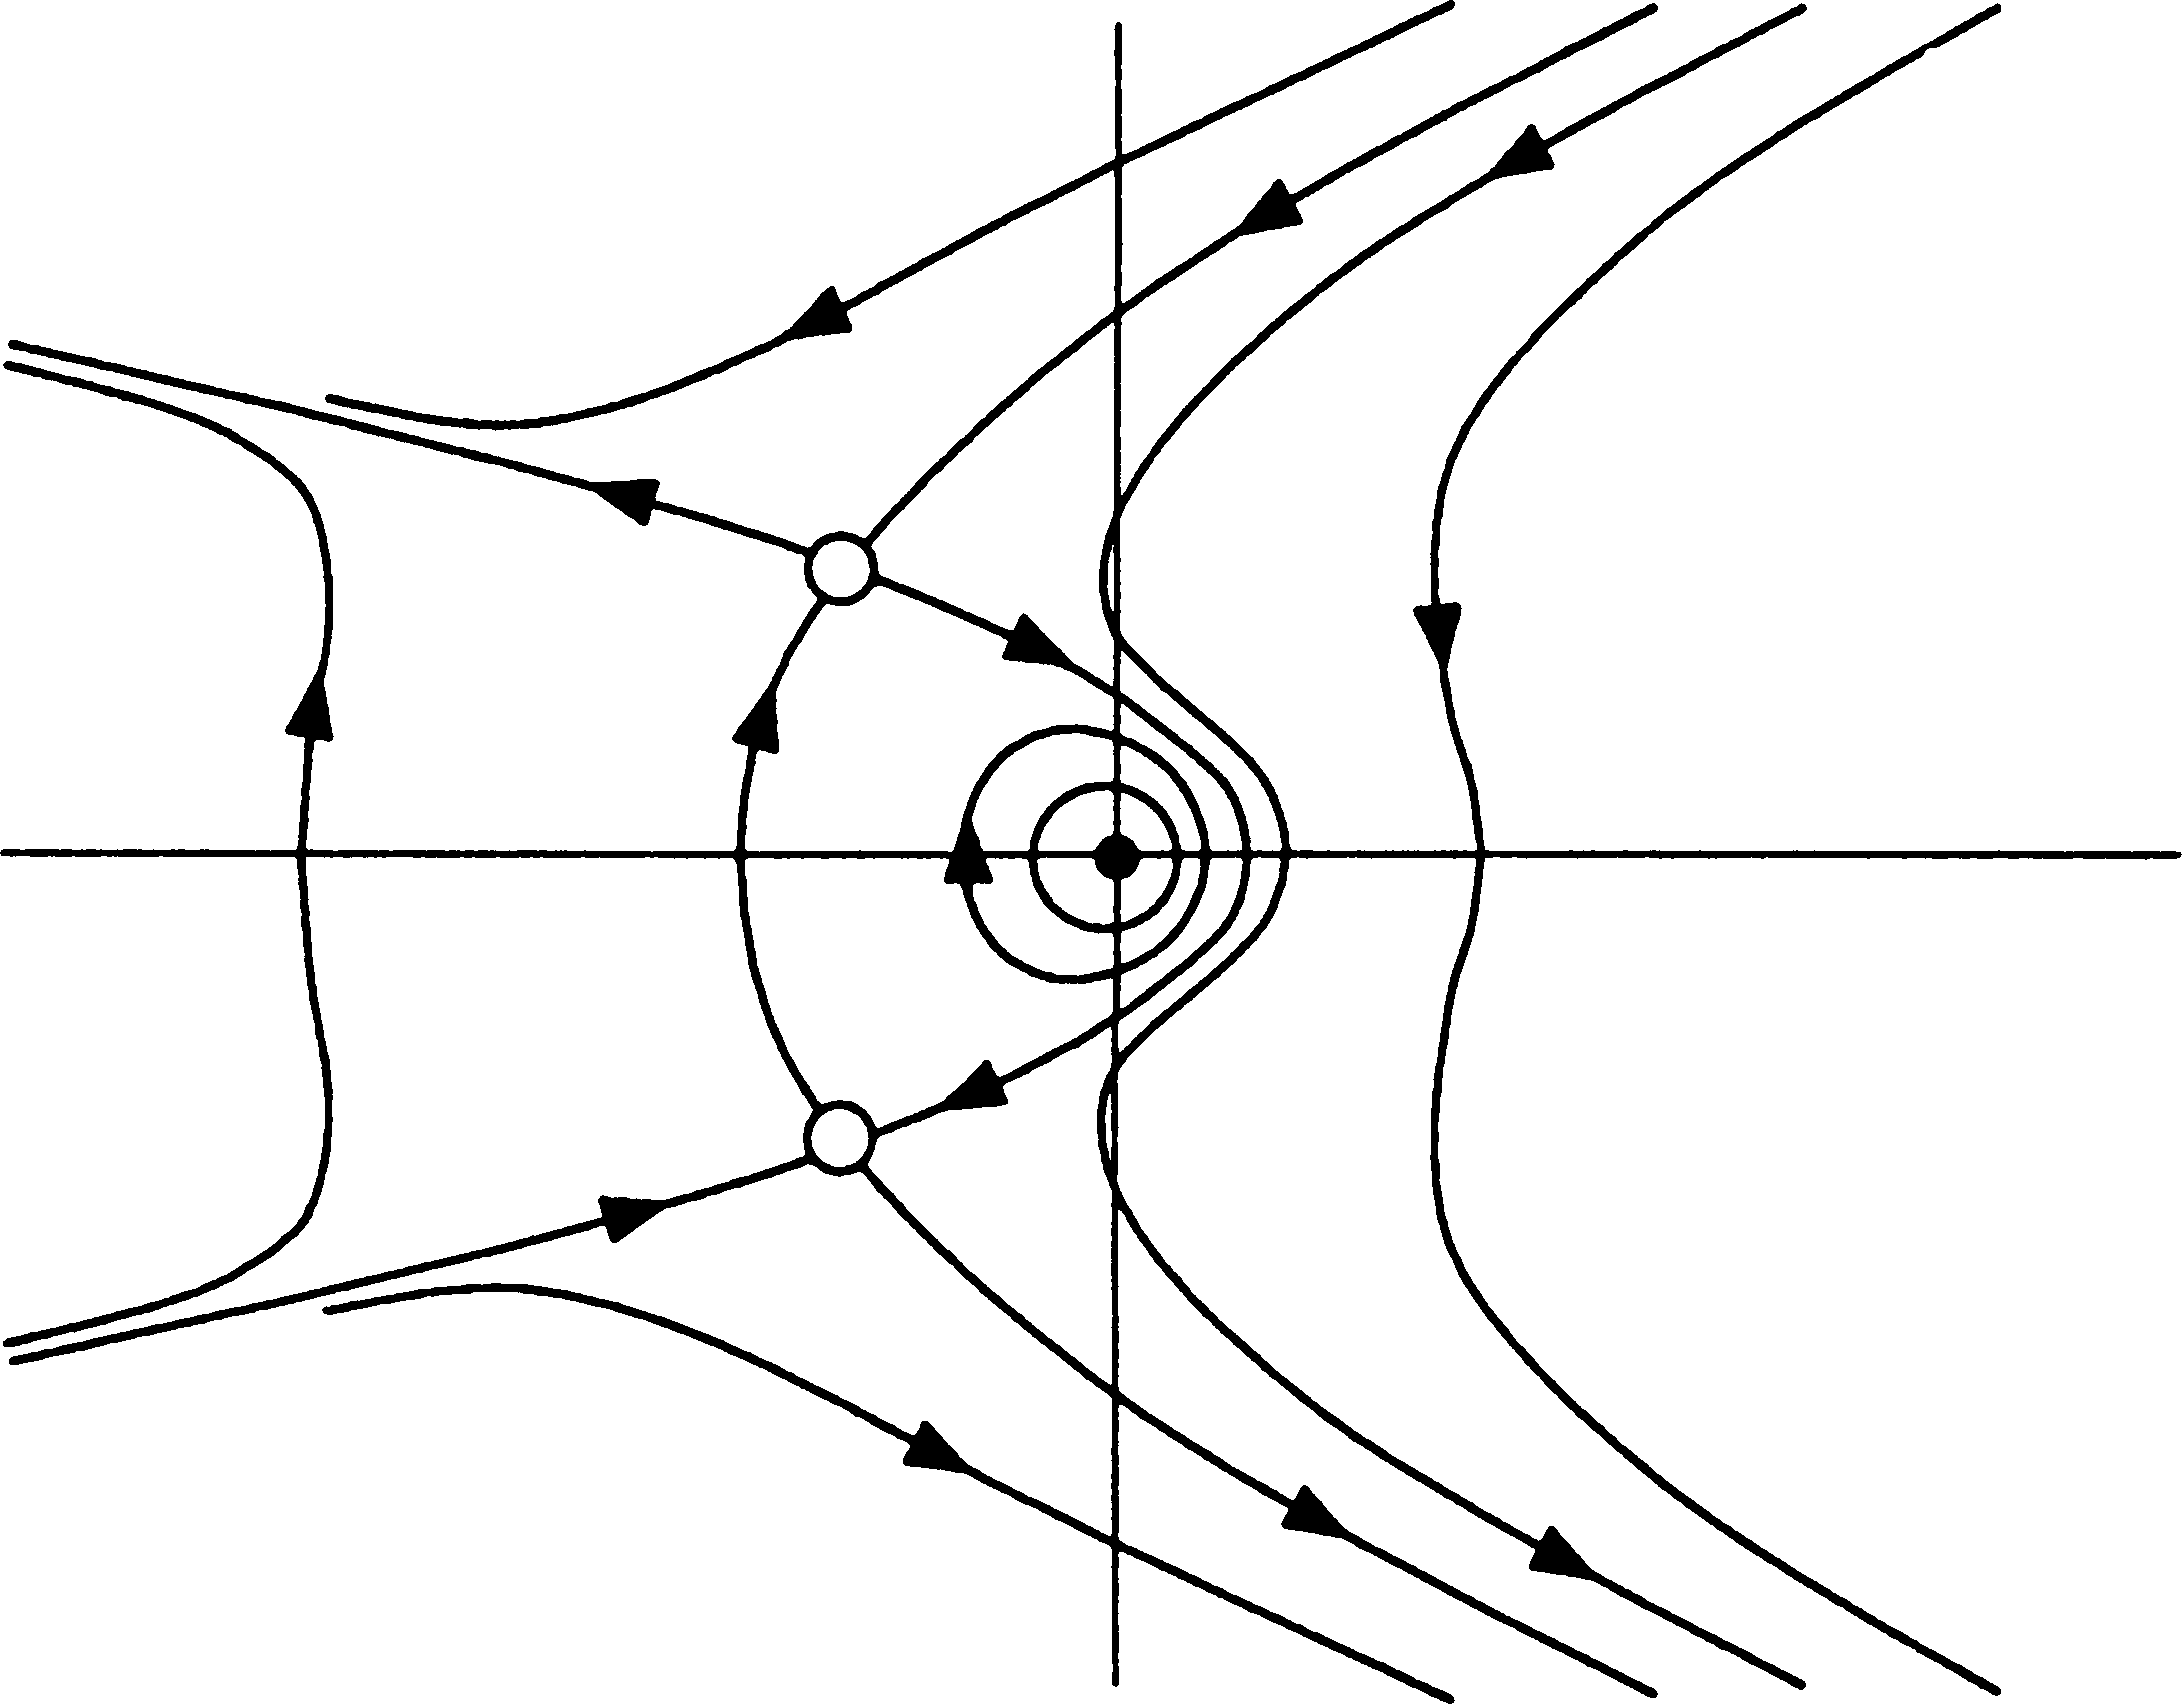
\includegraphics[width=0.82\textwidth]{images/Figures/figur-023.png}
\caption{Örnek 6.6.1 için tersinir sistemin faz portresi.}
\label{fig:6-6-4}
\end{figure}

İkiz eyer noktalarının bir yörünge çiftiyle bağlandığına dikkat ediniz. Bunlara heteroklinik yörüngeler ya da eyer bağlantıları denir. Homoklinik yörüngeler gibi, heteroklinik yörüngeler de tersinir veya korunumlu sistemlerde diğer sistemlere göre çok daha yaygındır.
\end{justify}

\subsection*{Örnek 6.6.2}
\addcontentsline{toc}{subsection}{Örnek 6.6.2}

\begin{justify}
Yalnızca tersinirlik argümanlarını kullanarak
\begin{align}
\dot{x} &= y,\\
\dot{y} &= x-x^2
\end{align}
sisteminin $x\ge 0$ yarı düzleminde bir homoklinik yörüngeye sahip olduğunu gösterelim.

\textbf{Çözüm.} Orijindeki eyer noktasının kararsız manifoldunu ele alalım. Lineerleştirme için kararsız özdoğrultu $(1,1)$ olduğundan, bu manifold orijini bu doğrultu boyunca terk eder. Bu nedenle orijine yakın bölgede kararsız manifoldun bir parçası birinci bölgede, yani $x,y>0$ bölgesinde yer alır.

Başlangıçta $\dot{x}=y>0$ olduğundan $x(t)$ artar. Ayrıca küçük $x$ için $\dot{y}=x-x^2>0$ olduğundan $y(t)$ de başlangıçta artar. Böylece faz noktası yukarı ve sağa doğru hareket eder. Yatay hızı artmaya devam ettiği için bir zamanda $x=1$ doğrusunu keser. Bundan sonra $\dot{y}<0$ olur ve $y(t)$ azalır; sonunda $y=0$ değerine ulaşır (Şekil~\ref{fig:6-6-5}).

Tersinirlik nedeniyle aynı uç noktalara sahip fakat oku ters yönde olan ikiz bir yörünge bulunmalıdır (Şekil~\ref{fig:6-6-6}). Bu iki yörünge birlikte istenen homoklinik yörüngeyi oluşturur.

\begin{figure}[H]
\centering
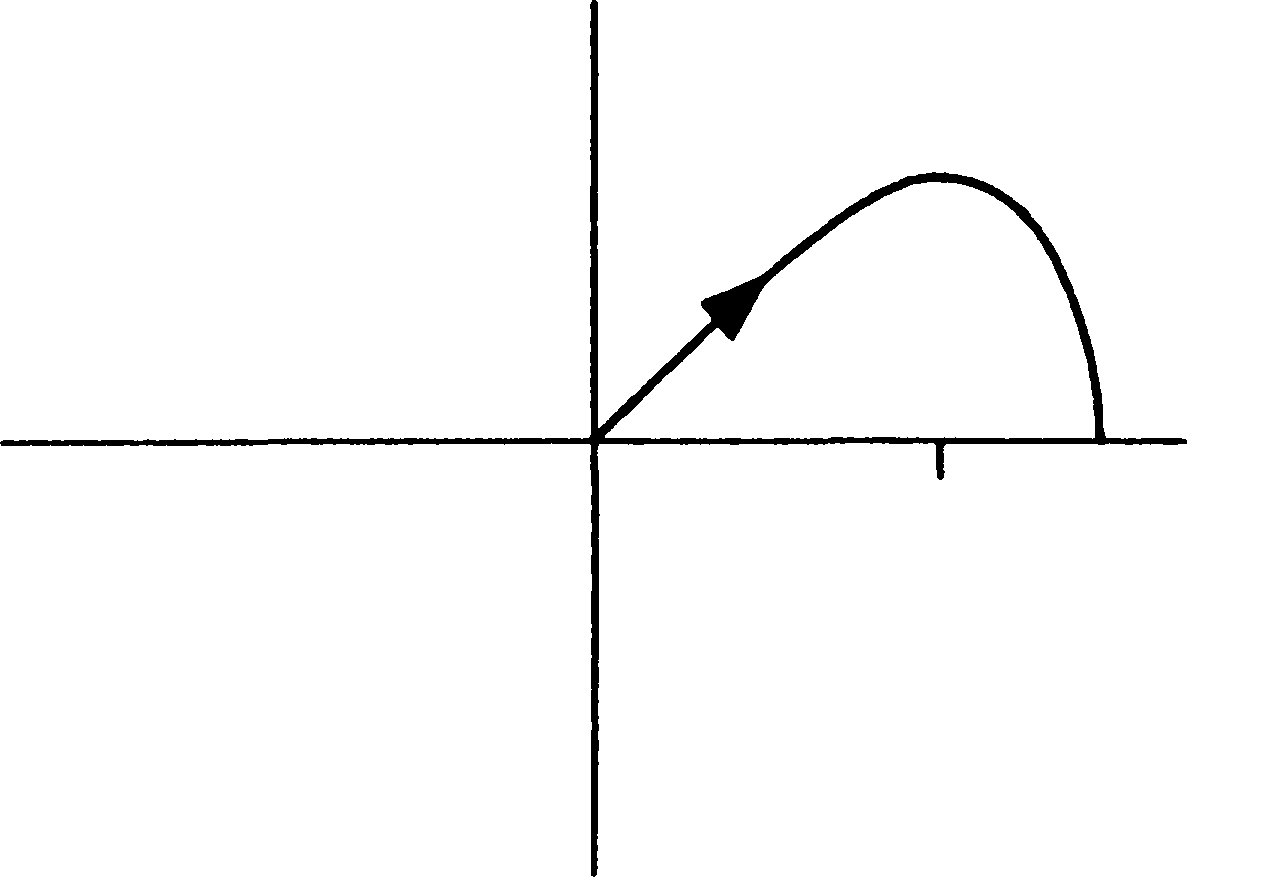
\includegraphics[width=0.82\textwidth]{images/Figures/figur-024.png}
\caption{Kararsız manifoldun $x=1$ doğrusunu kesip $y=0$ eksenine ulaşması.}
\label{fig:6-6-5}
\end{figure}
\begin{figure}[H]
\centering
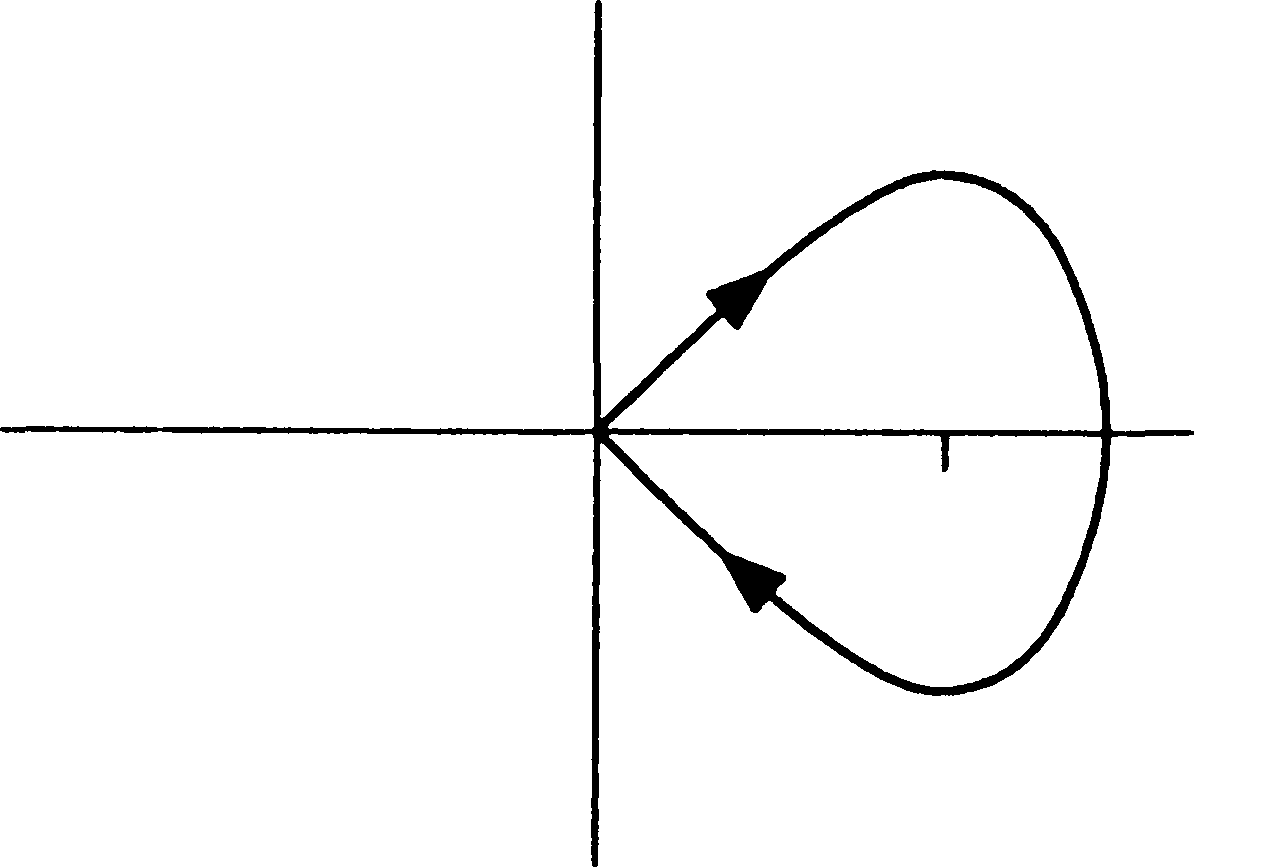
\includegraphics[width=0.82\textwidth]{images/Figures/figur-025.png}
\caption{Tersinirlik ile tamamlanan homoklinik yörünge.}
\label{fig:6-6-6}
\end{figure}
\end{justify}

\subsection*{Örnek 6.6.3}
\addcontentsline{toc}{subsection}{Örnek 6.6.3}

\begin{justify}
Aşağıdaki sistemin tersinir fakat korunumlu olmadığını gösterelim ve faz portresini çizelim:
\begin{align}
\dot{x} &= -2\cos x-\cos y,\\
\dot{y} &= -2\cos y-\cos x.
\end{align}

\textbf{Çözüm.} Sistem $t\mapsto -t$, $x\mapsto -x$ ve $y\mapsto -y$ değişken dönüşümleri altında değişmez. Bu nedenle $R(x,y)=(-x,-y)$ dönüşümüyle tersinirdir.

Sistemin korunumlu olmadığını göstermek için çekici bir sabit noktasının olduğunu göstermek yeterlidir. Sabit noktalar
\begin{equation}
2\cos x=-\cos y, \qquad 2\cos y=-\cos x
\end{equation}
koşullarını sağlar. Bu denklemler birlikte çözülünce $\cos x^{*}=\cos y^{*}=0$ bulunur. Böylece dört sabit nokta vardır:
\begin{equation}
(x^{*},y^{*})=\left(\pm\frac{\pi}{2},\pm\frac{\pi}{2}\right).
\end{equation}
$(-\pi/2,-\pi/2)$ noktasının çekici olduğunu gösterelim. Bu noktadaki Jacobian
\begin{equation}
A=\begin{pmatrix}
2\sin x^{*} & \sin y^{*}\\
\sin x^{*} & 2\sin y^{*}
\end{pmatrix}
=
\begin{pmatrix}-2&-1\\-1&-2\end{pmatrix}
\end{equation}
olur. Burada $\tau=-4$, $\Delta=3$ ve $\tau^2-4\Delta=4$ olduğundan sabit nokta kararlı düğümdür. Bu, sistemin korunumlu olmadığını gösterir.

Diğer üç sabit noktanın biri kararsız düğüm, ikisi ise eyer noktasıdır. Faz portresi Şekil~\ref{fig:6-6-7}'de gösterilecektir. Tersinirlik simetrisi, $(x,y)$ ve $R(x,y)=(-x,-y)$ noktalarındaki dinamiklerin aynı görünmesi fakat ok yönlerinin ters olmasıdır.

\begin{figure}[H]
\centering
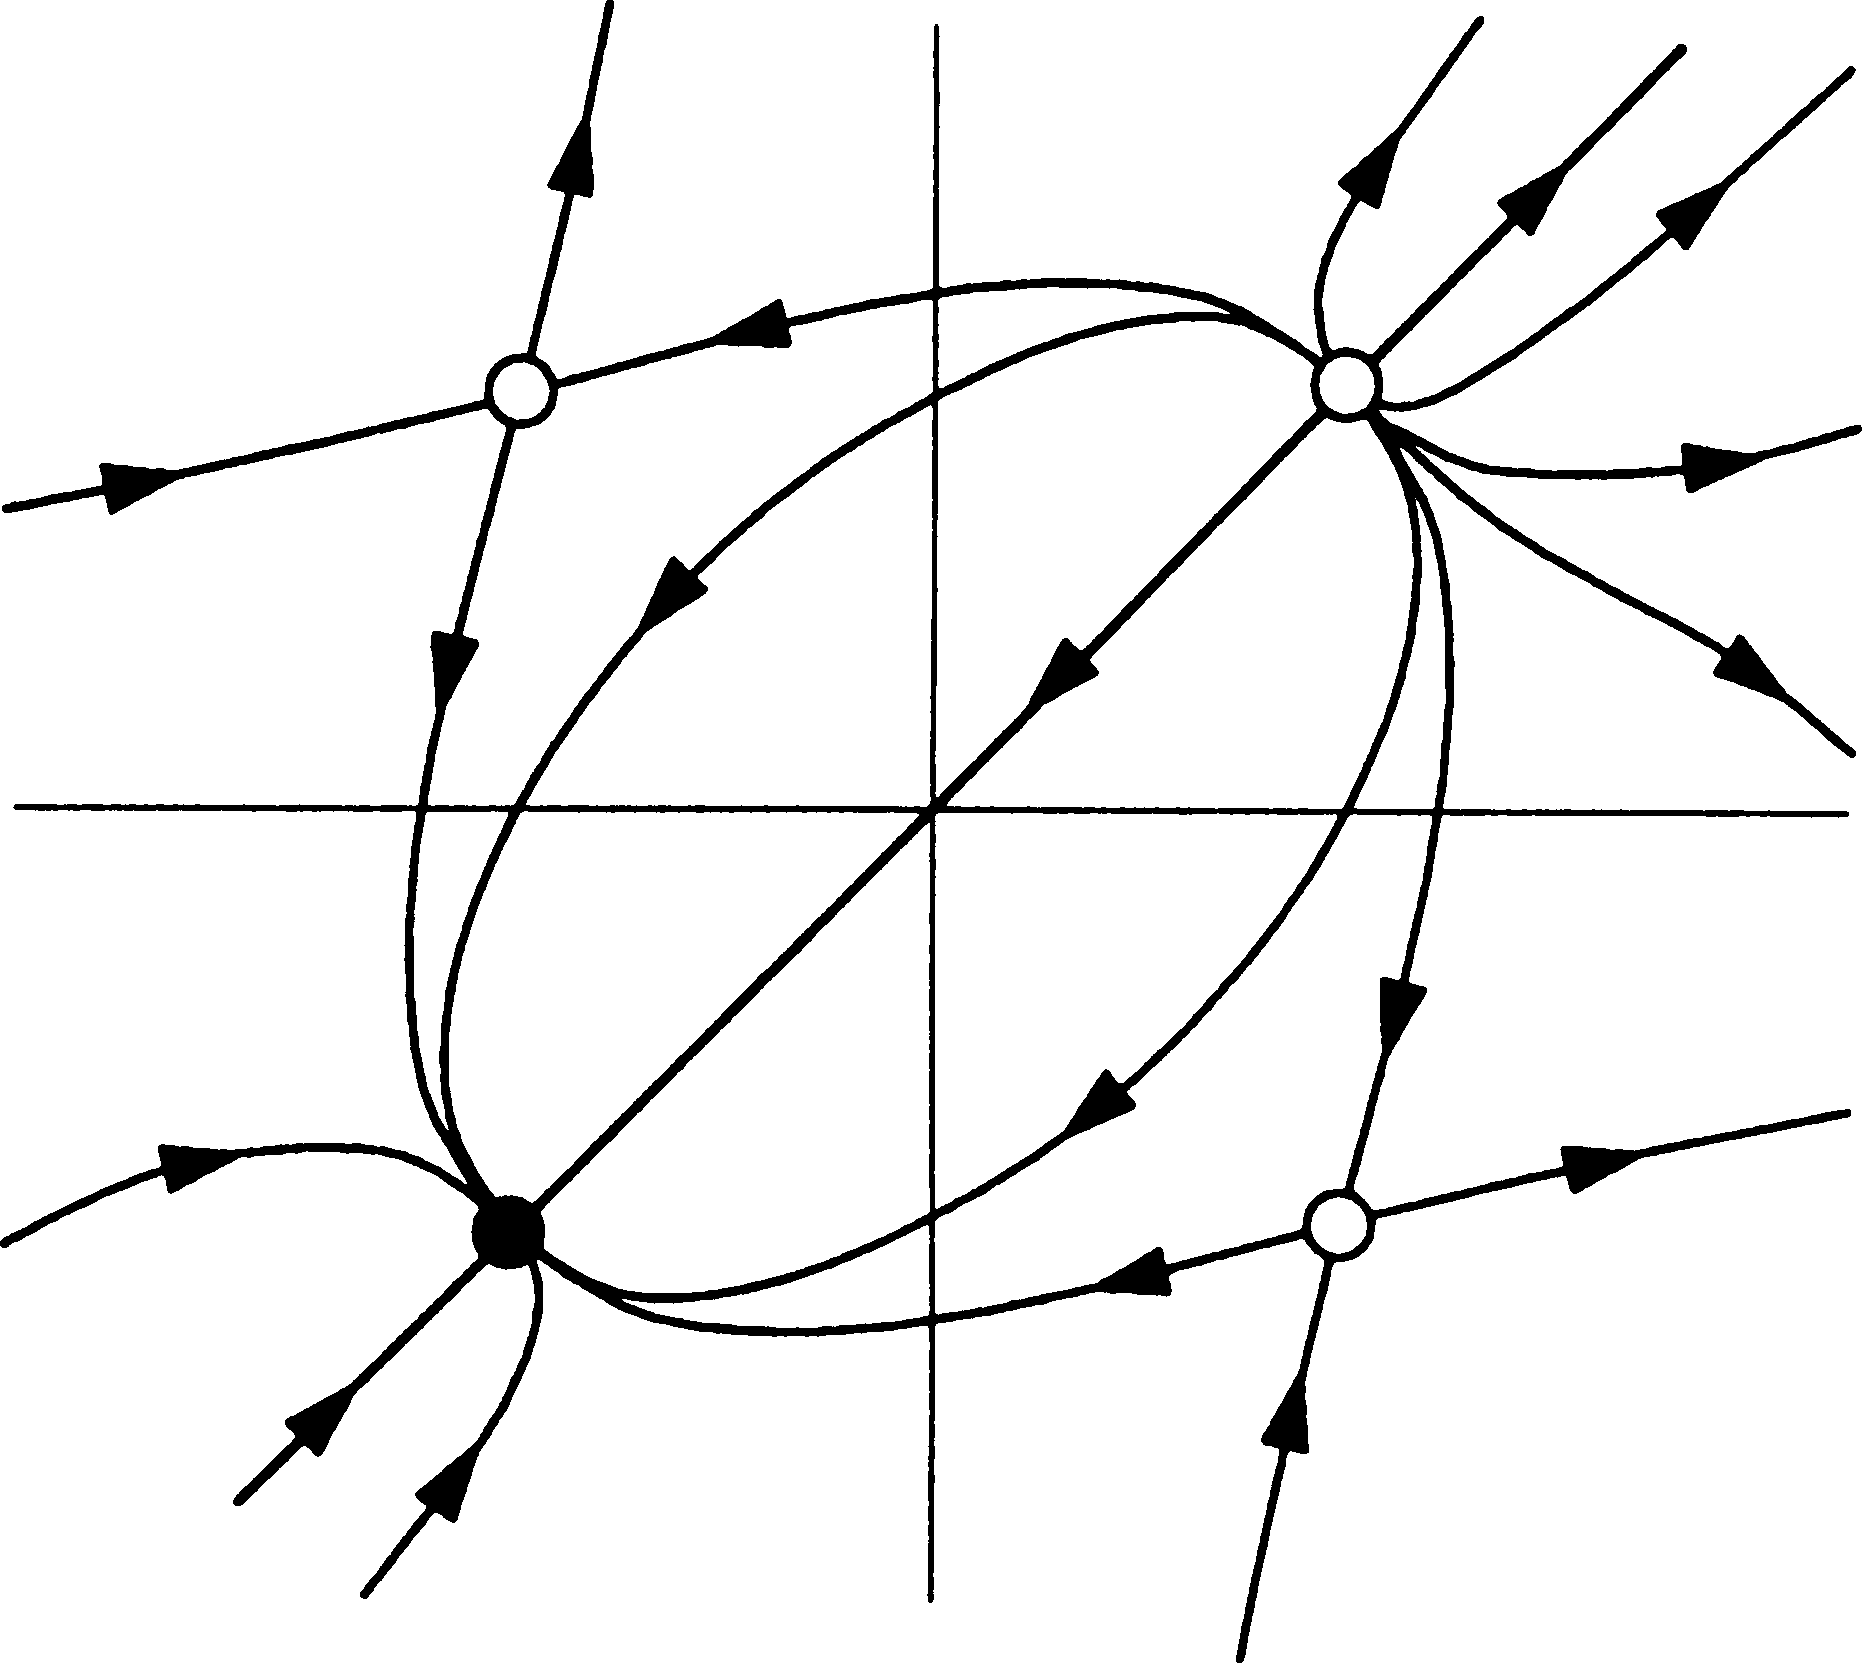
\includegraphics[width=0.82\textwidth]{images/Figures/figur-026.png}
\caption{Tersinir fakat korunumlu olmayan sistemin faz portresi.}
\label{fig:6-6-7}
\end{figure}
\end{justify}

\newpage